\section{Constituci�n del Plan de Estudios}\label{sec:courses-by-semester}
Esta propuesta puede ser analizada por el n�mero de cr�ditos dedicados a cada �rea
%horas de clase de las mismas
y por niveles de cursos (Introductorios, Intermedios, Avanzados y Proyectos).
\vspace{0.5cm}

\begin{figure}[h!]
      \centering
      \includegraphics[width=10cm]{\OutputFigDir/pie-credits}
      \label{fig:pie-credits}
      \caption{Distribuci�n de cursos por �reas considerando creditaje.}
\end{figure}

% \input{\OutputTexDir/distribution-area-by-semester}
\input{\OutputTexDir/distribution-credits-by-area-by-semester}

\begin{figure}[h!]
      \centering
      \includegraphics[width=10cm]{\OutputFigDir/pie-by-levels}
      \label{fig:pie-niveles}
      \caption{Distribuci�n de cr�ditos por niveles de cursos.}
\end{figure} %Graphics by level, by area, etc

\begin{landscape}
La relaci�n de cursos se muestra a continuaci�n:
\input{\OutputTexDir/tables-by-semester}

\OnlySPC{Es importante resaltar que todos los semestres podr�an ser completados con cursos extras de acuerdo al perfil de la instituci�n.}
\end{landscape}

\begin{landscape}
\section{Requisitos de cursos}
\vspace{-0.3cm}Los requisitos de cada curso pueden ser observados en la secci�n~\ref{sec:courses-by-semester} (P�g.~\pageref{sec:courses-by-semester}) y de forma gr�fica a continuaci�n.
\begin{figure}[h!]
      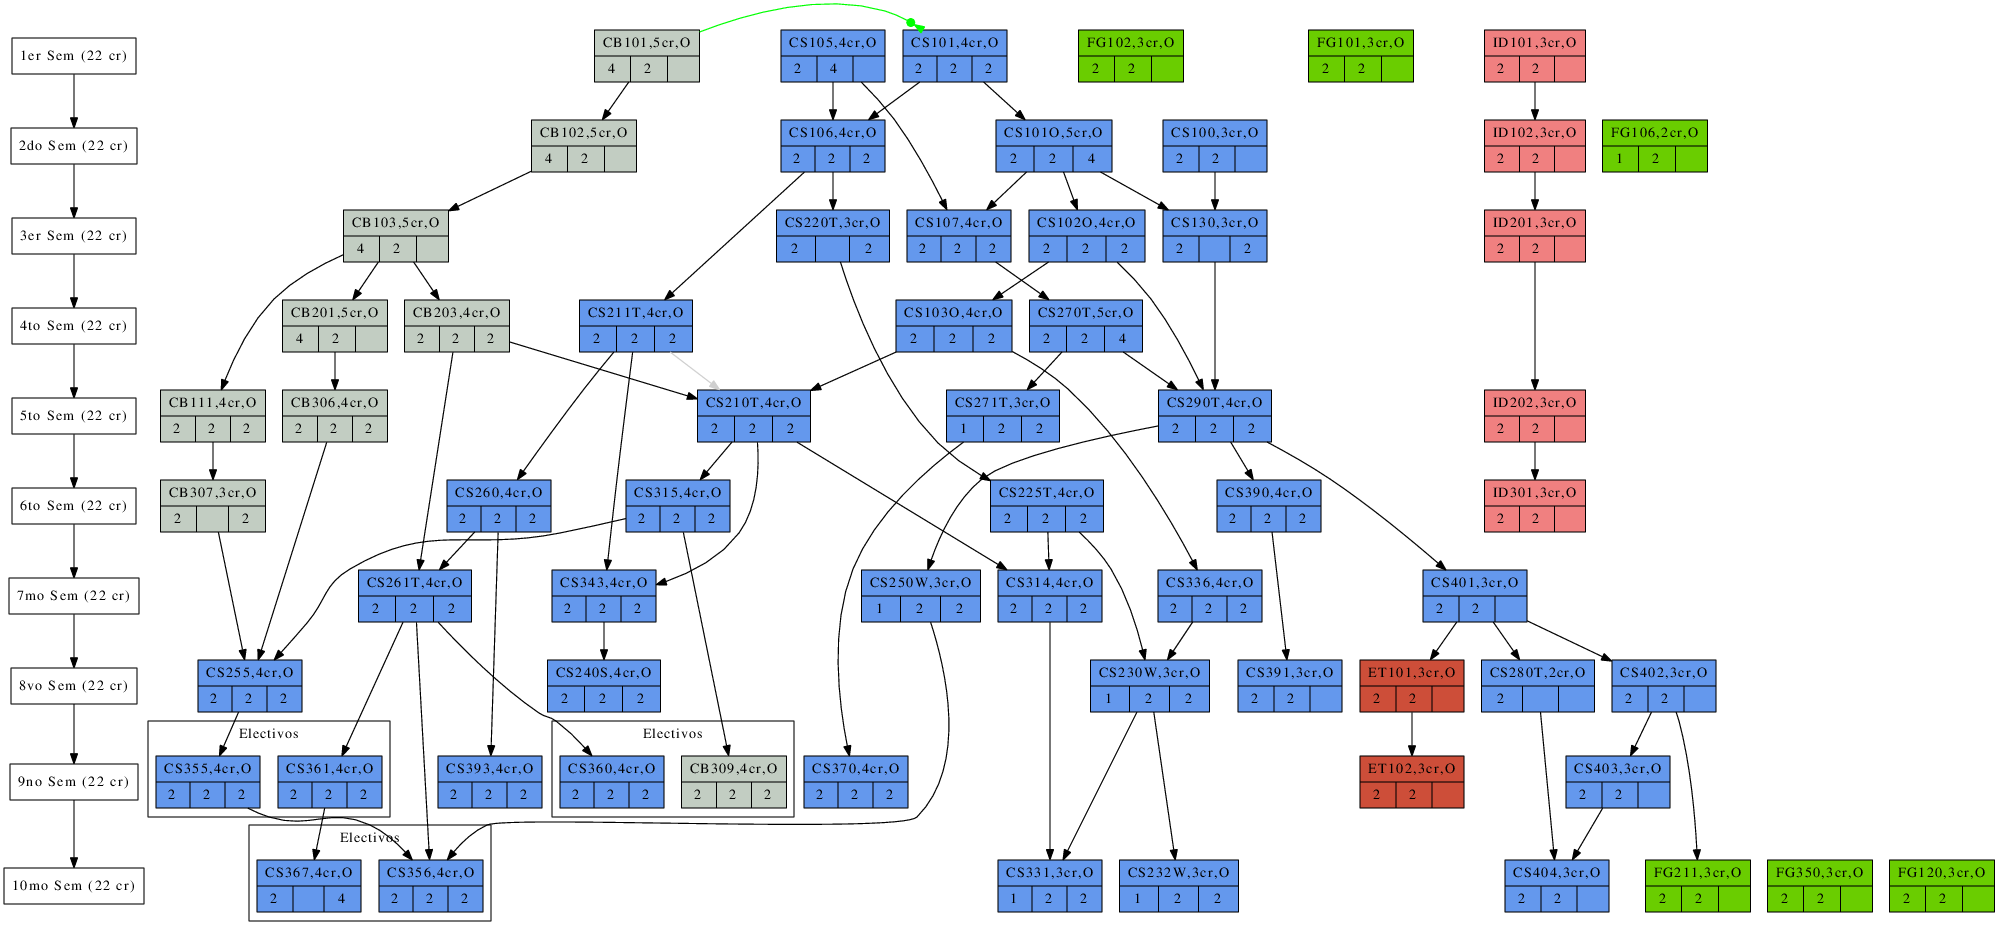
\includegraphics[width=23cm]{\OutputFigDir/small-graph-curricula.ps}
      \label{fig:small-curricula}
      \caption{Malla curricular \SchoolFullName}
\end{figure}
\end{landscape}


